\documentclass[11pt]{article}
\usepackage[margin=1in]{geometry}
\usepackage{graphicx}
\usepackage{float}
\usepackage{caption}
\usepackage{subcaption}
\usepackage{amsmath}
\usepackage{hyperref}

\title{CSCI 566 - Assignment 2\\ \Large Problem 1 Solution}
\author{Zishun Liu / 7285815424}
\date{\today}

\begin{document}

\maketitle

\section{Auto-Encoder Samples \& Inline Question}

\subsection{Auto-Encoder Samples}

\begin{figure}[H]
    \centering
    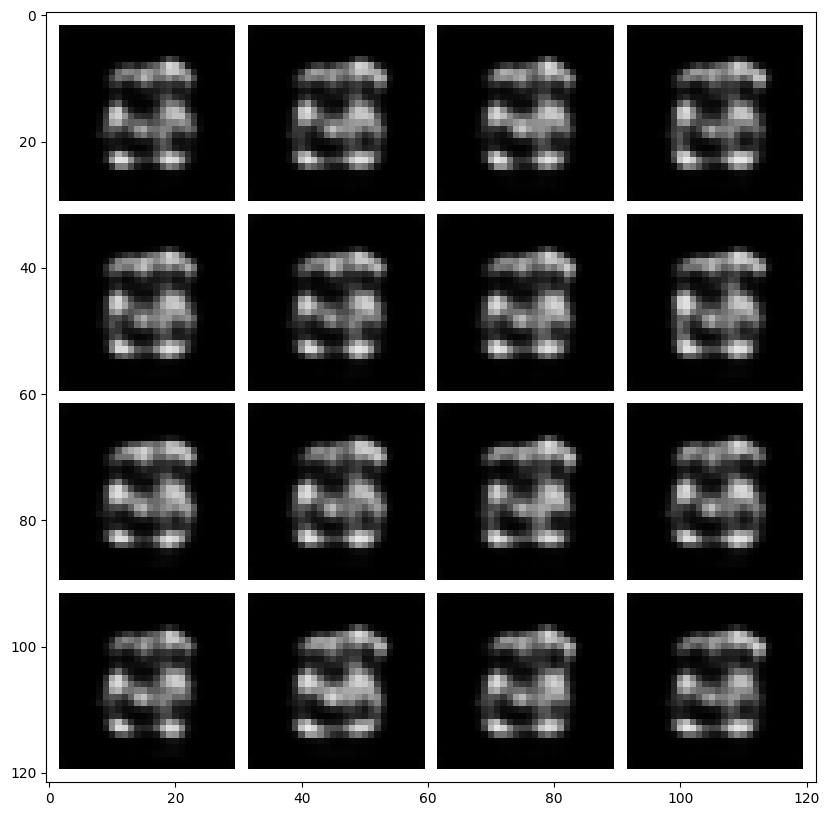
\includegraphics[width=0.6\linewidth]{ae_samples.png}
    \caption{Samples generated from the deterministic Auto-Encoder.}
\end{figure}

\subsection{Inline Question}
\textbf{Question:}  Describe your observations, why do you think they occur? [2pt] 

\textbf{Answer:} The decoded samples generally look like meaningless noise or blurry blobs, rarely resembling clear digits. This occurs because the deterministic Auto-Encoder does not regularize its latent space. It maps training inputs to arbitrary points in the latent space simply to minimize reconstruction error, leaving vast regions of the latent space "empty" or undefined. When we sample randomly from a unit Gaussian prior, we are likely picking points from these untrained, arbitrary regions, causing the decoder to output nonsensical images.

\newpage
\section{VAE Training Curves, Reconstructions, and Samples}

\subsection{Case 1: $\beta = 0$}

\begin{figure}[H]
    \centering
    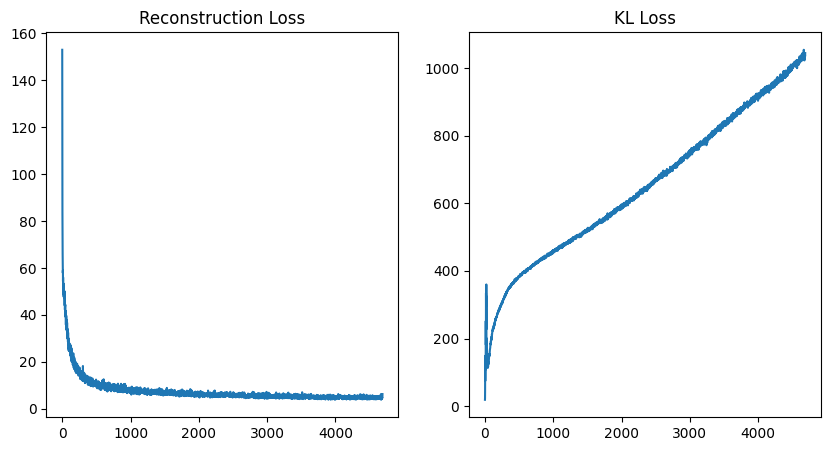
\includegraphics[width=0.5\linewidth]{vae_beta0_curve.png}
    \caption{Training curve for $\beta = 0$.}
\end{figure}
\begin{figure}[H]
    \centering
    \begin{subfigure}{0.48\textwidth}
        \centering
        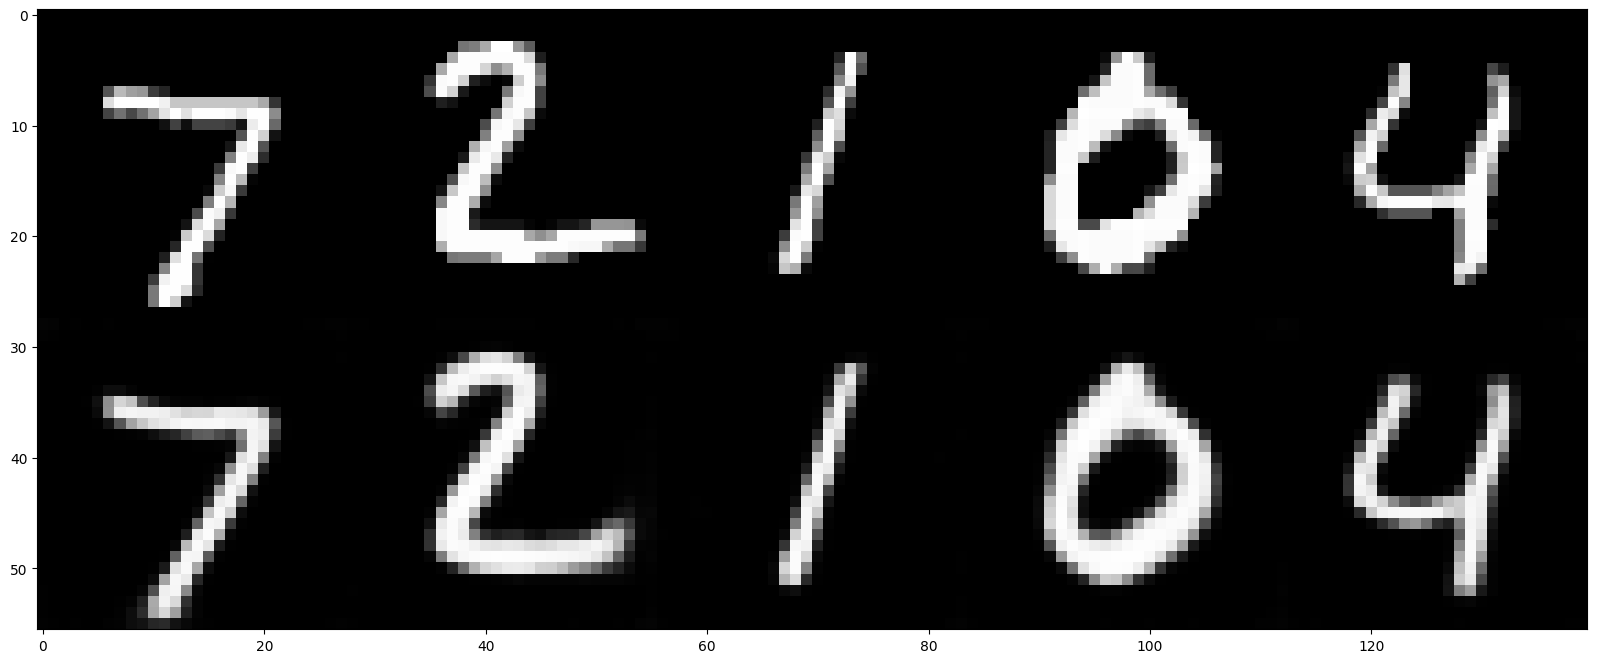
\includegraphics[width=\linewidth]{vae_beta0_rec.png}
        \caption{Reconstructions ($\beta = 0$)}
    \end{subfigure}
    \hfill
    \begin{subfigure}{0.48\textwidth}
        \centering
        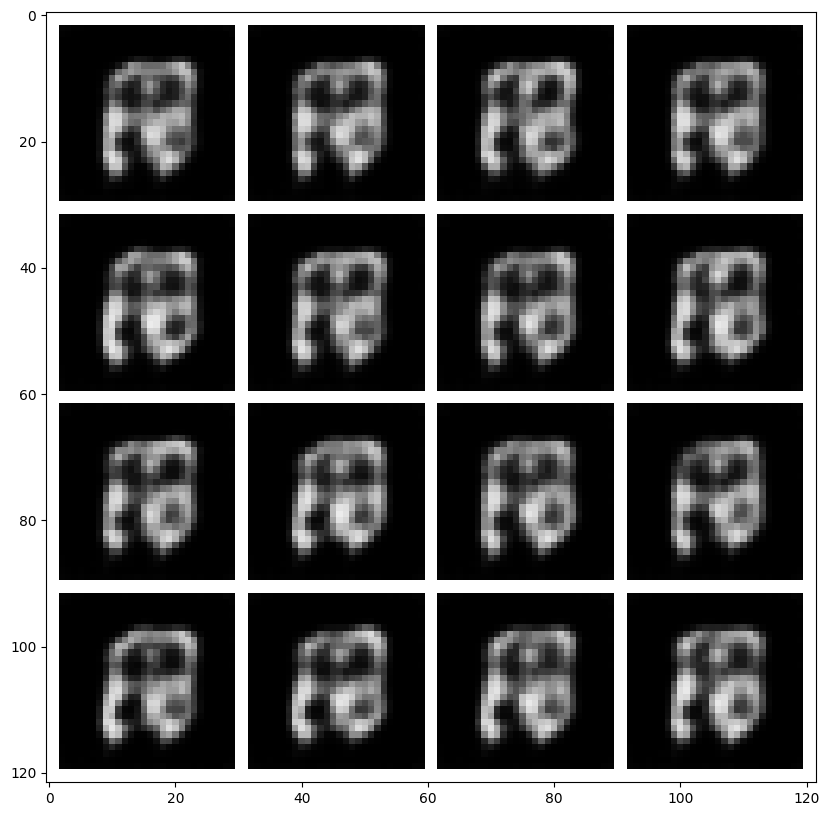
\includegraphics[width=\linewidth]{vae_beta0_samples.png}
        \caption{Samples ($\beta = 0$)}
    \end{subfigure}
    \caption{Reconstructions and samples for $\beta = 0$.}
\end{figure}

\subsection{Case 2: $\beta = 10$}

\begin{figure}[H]
    \centering
    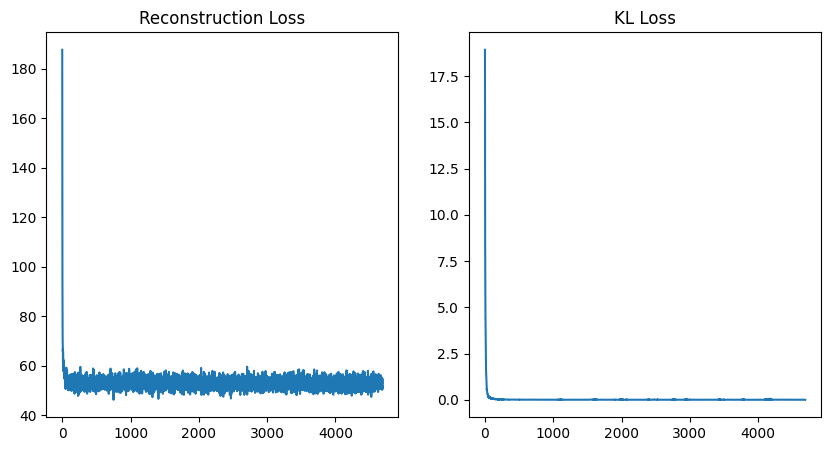
\includegraphics[width=0.5\linewidth]{vae_beta10_curve.png}
    \caption{Training curve for $\beta = 10$.}
\end{figure}
\begin{figure}[H]
    \centering
    \begin{subfigure}{0.48\textwidth}
        \centering
        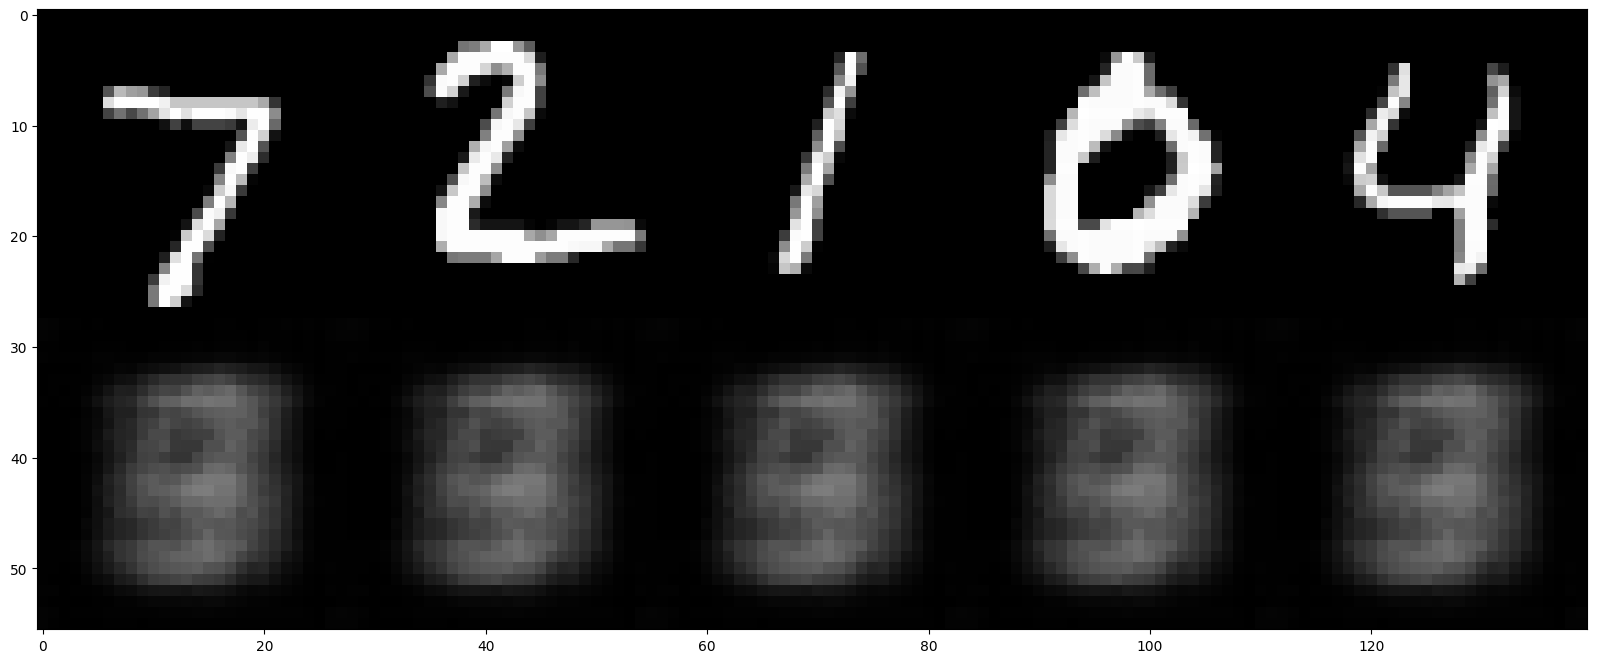
\includegraphics[width=\linewidth]{vae_beta10_rec.png}
        \caption{Reconstructions ($\beta = 10$)}
    \end{subfigure}
    \hfill
    \begin{subfigure}{0.48\textwidth}
        \centering
        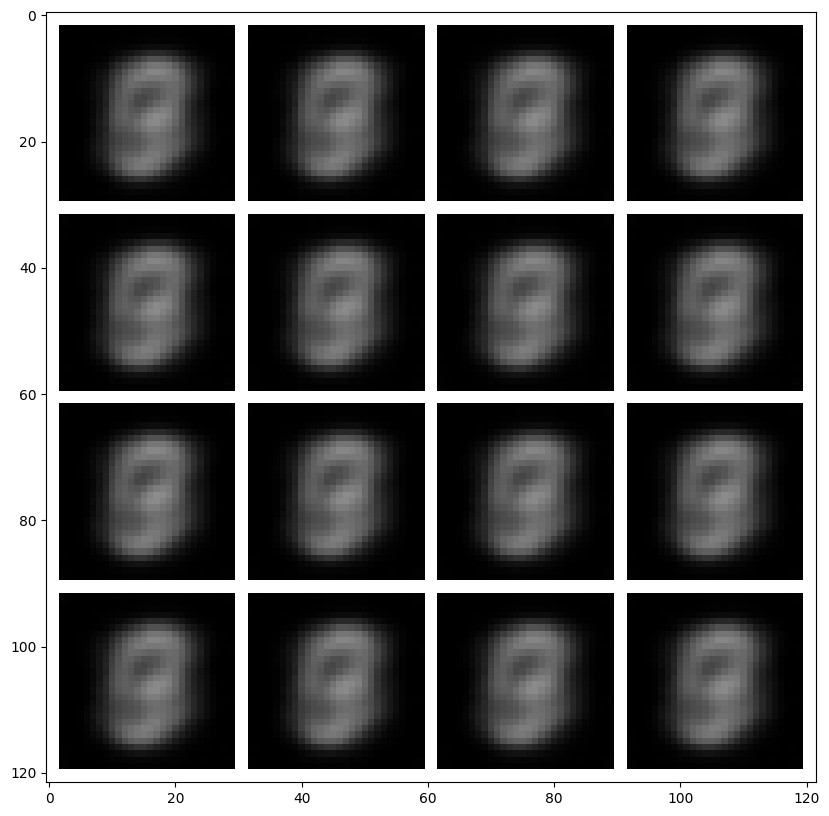
\includegraphics[width=\linewidth]{vae_beta10_samples.png}
        \caption{Samples ($\beta = 10$)}
    \end{subfigure}
    \caption{Reconstructions and samples for $\beta = 10$.}
\end{figure}

\subsection{Case 3: Tuned $\beta$}
\textbf{Tuned value used for $\beta$:} 1.0 

% PLEASE SAVE YOUR TUNED BETA PLOTS AS 'vae_betatuned_curve.png', 'vae_betatuned_rec.png', 'vae_betatuned_samples.png'
\begin{figure}[H]
    \centering
    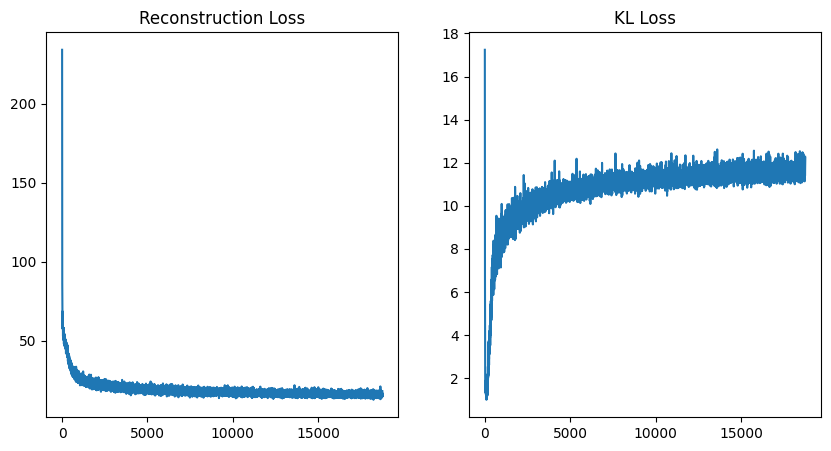
\includegraphics[width=0.5\linewidth]{vae_betatuned_curve.png}
    \caption{Training curve for tuned $\beta$.}
\end{figure}
\begin{figure}[H]
    \centering
    \begin{subfigure}{0.48\textwidth}
        \centering
        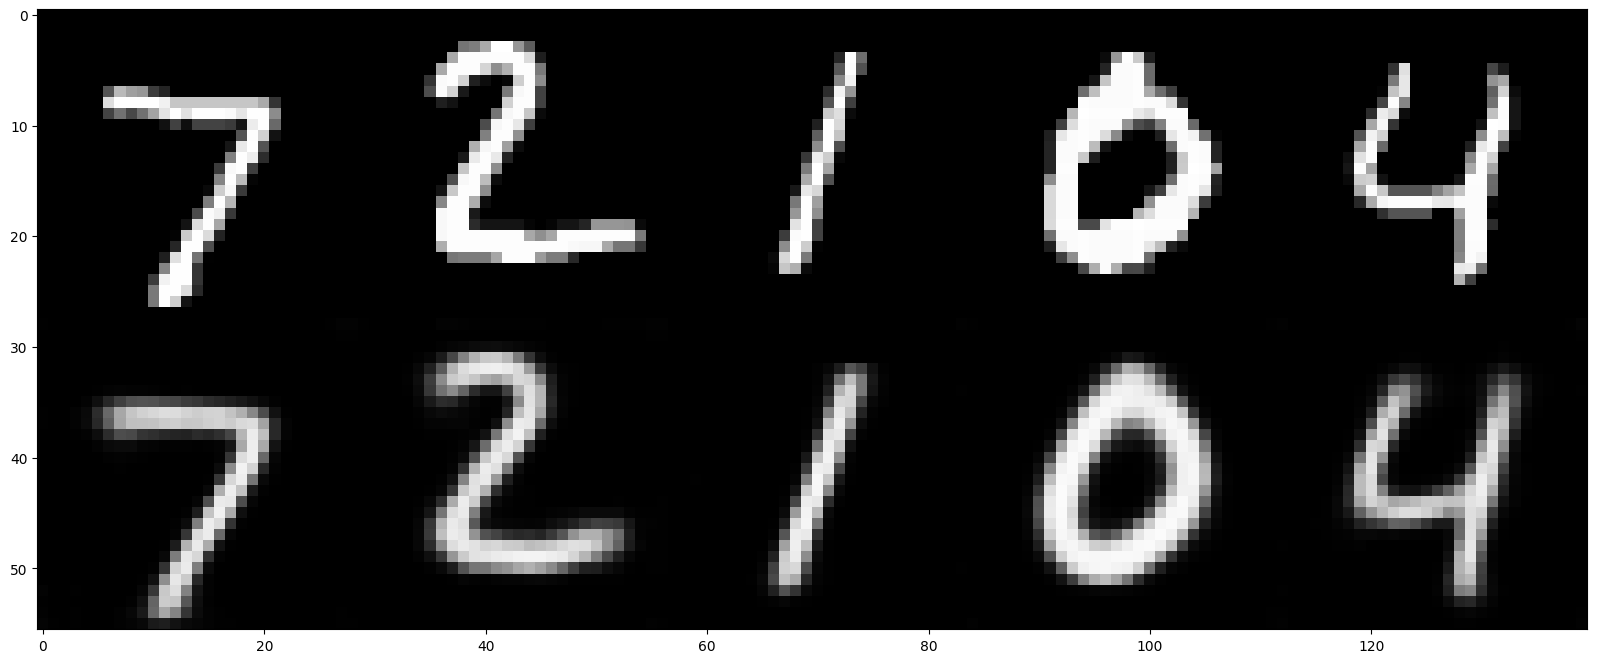
\includegraphics[width=\linewidth]{vae_betatuned_rec.png}
        \caption{Reconstructions (Tuned $\beta$)}
    \end{subfigure}
    \hfill
    \begin{subfigure}{0.48\textwidth}
        \centering
        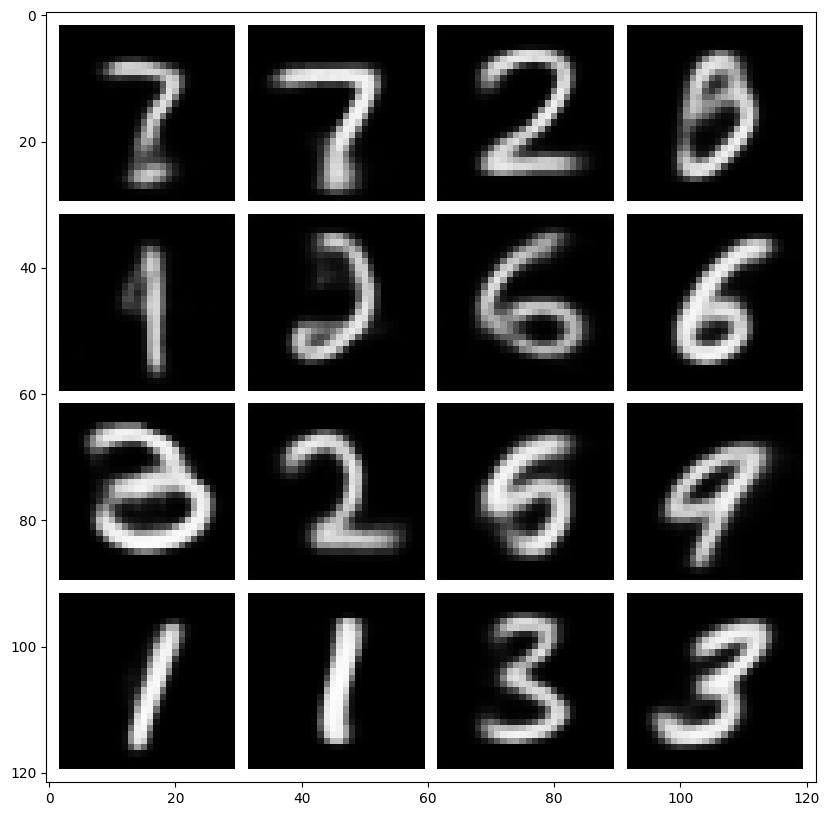
\includegraphics[width=\linewidth]{vae_betatuned_samples.png}
        \caption{Samples (Tuned $\beta$)}
    \end{subfigure}
    \caption{Reconstructions and samples for tuned $\beta$.}
\end{figure}

\newpage
\section{Answers to VAE Inline Questions}

\textbf{What can you observe when setting  $\beta=0$ ? Explain your observations! [3pt]}

\textbf{Answer:} The reconstructions are sharp and highly accurate, but the randomly generated samples still look like meaningless blobs. Setting $\beta = 0$ completely zeroes out the KL divergence penalty, removing all regularization from the posterior distribution. The model effectively collapses back into a standard, deterministic Auto-Encoder. Because the latent space is not forced to approximate a unit Gaussian prior $\mathcal{N}(0, I)$, sampling from that prior pulls from undefined regions, resulting in failed generations.

\vspace{1em}
\textbf{What can you observe when setting $\beta = 10$? Explain your observations![3pt]}

\textbf{Answer:} The reconstructions become extremely blurry, and the random samples look like uniform blobs or a generic average of all digits, completely lacking distinct features. Setting $\beta$ this high over-regularizes the model. The KL divergence penalty dominates the objective function, forcing the encoder to map almost every input to the exact same unit Gaussian prior at the severe expense of the reconstruction error. Because all inputs are squashed into the same region with mean 0 and variance 1, the decoder is starved of any specific latent information. As a result, it fails to distinguish between different digits and collapses into predicting a blurry, uninformative average.

\vspace{1em}
\textbf{Characterize what properties you would expect for reconstructions (1pt) and samples (2pt) of a well-tuned VAE! [3pt] }

\textbf{Answer:} 
\begin{itemize}
    \item \textbf{Reconstructions:} They should be identifiable and reasonably accurate to the input, though slightly blurrier than those of a deterministic Auto-Encoder. This slight blur is a natural byproduct of the reparametrization trick injecting noise during training to enforce the continuous latent distribution.
    \item \textbf{Samples:} They should look like realistic, diverse, and well-formed digits. Because a well-tuned $\beta$ successfully balances reconstruction with latent regularization, the model ensures there are no "dead zones" in the embedding space. Drawing a random sample from $\mathcal{N}(0, I)$ lands in a meaningful, well-structured region that the decoder knows how to translate into a coherent image.
\end{itemize}

\newpage
\section{Interpolation Comparisons \& Inline Question}

\subsection{Representative Interpolation Comparisons}
% PLEASE SAVE YOUR 3 INTERPOLATION PLOTS AS 'interp_1.png', 'interp_2.png', 'interp_3.png'
% Each image should ideally show the AE interpolation row and the VAE interpolation row for the same start/end images.
\begin{figure}[H]
    \centering
    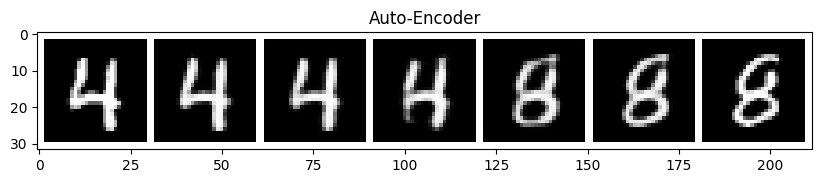
\includegraphics[width=0.8\linewidth]{interp_1.png}
    \caption{Interpolation Comparison 1 (Top: AE, Bottom: VAE)(from 4 to 8)}
\end{figure}
\begin{figure}[H]
    \centering
    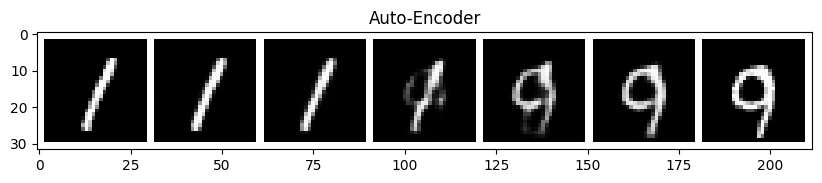
\includegraphics[width=0.8\linewidth]{interp_2.png}
    \caption{Interpolation Comparison 2 (Top: AE, Bottom: VAE)(from 1 to 9)}
\end{figure}
\begin{figure}[H]
    \centering
    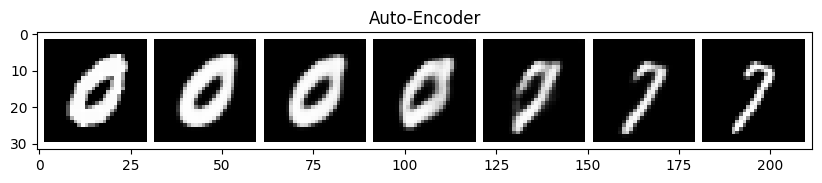
\includegraphics[width=0.8\linewidth]{interp_3.png}
    \caption{Interpolation Comparison 3 (Top: AE, Bottom: VAE)(from 0 to 7)}
\end{figure}

\subsection{Interpolation Inline Question}
\textbf{Question:} How do AE and VAE embedding space interpolations differ? How do you expect these differences to affect downstream learning?

\textbf{Answer:} 
\begin{itemize}
    \item \textbf{Differences:} In the deterministic AE, interpolating between two digits often results in a disjointed visual transition. The starting digit fades out while the ending digit fades in, passing through noisy, unrealistic "ghost" states. In contrast, the VAE's interpolation is much smoother and structurally continuous. The shapes physically morph into one another (e.g., the loop of a 4 smoothly opening up into an 8), with intermediate steps often looking like plausible, albeit ambiguous, handwritten characters.
    \item \textbf{Impact on Downstream Learning:} The VAE's smooth interpolation proves its latent space is dense, continuous, and semantic. It has successfully learned underlying generative factors (like stroke width, loop presence, and angle) rather than simply memorizing data points. For downstream tasks like classification or clustering, this highly structured representation is vastly superior. Similar data points naturally cluster together, and the model is much more robust to noise or variations. Conversely, the AE's fragmented latent space means that small, unseen perturbations could lead to unpredictable results, making downstream models more brittle and prone to overfitting.
\end{itemize}

\end{document}